% Candidate source: src-e83c48821eaac4546df1607aa7bd47f8c49362fe9d091f3ff8accf356722e61c
% Source PDF SHA-256: 0a787b530b939cb104a802de2c27119b5d150bac7c4f0e78b069bc103f381232
% PDF page 2 (printed page 207), question 22.
% Redraw follows visible relations: triangle OBC with recursive midpoint sequence P1, P2, P3, P4, P5.
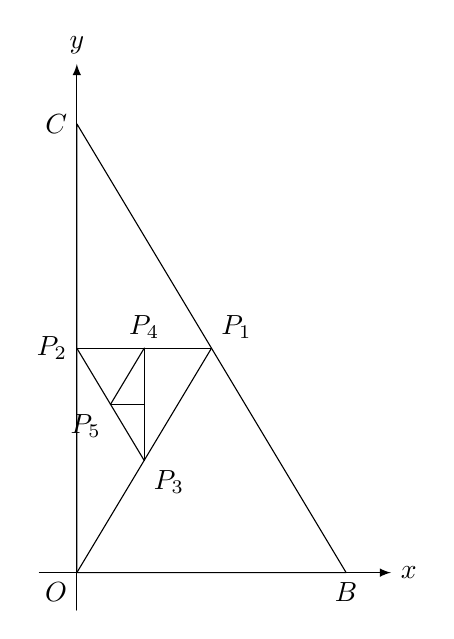
\begin{tikzpicture}[line cap=round,line join=round,>=latex,scale=0.95]
  % Coordinates for triangle OBC
  \coordinate (O) at (0,0);
  \coordinate (B) at (3.6,0);
  \coordinate (C) at (0,6.0);

  % Coordinates for midpoints P1 to P6
  \coordinate (P1) at (1.8,3.0);
  \coordinate (P2) at (0,3.0);
  \coordinate (P3) at (0.9,1.5);
  \coordinate (P4) at (0.9,3.0);
  \coordinate (P5) at (0.45,2.25);
  \coordinate (P6) at (0.9,2.25);

  % Axes
  \draw[->] (-0.5,0) -- (4.2,0) node[right] {$x$};
  \draw[->] (0,-0.5) -- (0,6.8) node[above] {$y$};

  % Triangle OBC
  \draw (C) -- (B) -- (O) -- cycle;

  % Spiral midpoint segments
  \draw (O) -- (P1);
  \draw (P1) -- (P2);
  \draw (P2) -- (P3);
  \draw (P3) -- (P4);
  \draw (P4) -- (P5);
  \draw (P5) -- (P6);

  % Labels
  \node[below left] at (O) {$O$};
  \node[below] at (B) {$B$};
  \node[left] at (C) {$C$};
  \node[above right] at (P1) {$P_1$};
  \node[left] at (P2) {$P_2$};
  \node[below right] at (P3) {$P_3$};
  \node[above] at (P4) {$P_4$};
  \node[below left] at (P5) {$P_5$};
\end{tikzpicture}
